\begin{figure}
    \centering
    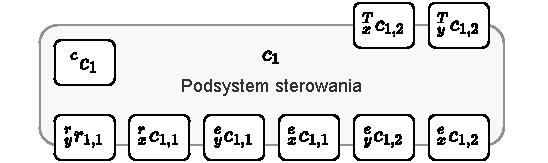
\includegraphics[width=\columnwidth]{figures/ISR-cs-model.pdf}
    \label{fig:model-cs}
    \caption{Struktura ogólna podsystemu sterowania}
\end{figure}

\begin{figure}
    \centering
    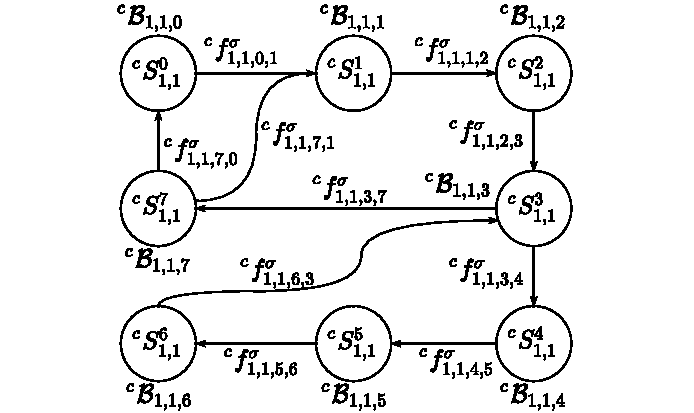
\includegraphics[width=\columnwidth]{figures/ISR-cs-behaviours.pdf}
    \label{fig:zachowania-cs}
    \caption{Automat zachowań podsystemu sterowania}
\end{figure}

Zachowania:
\begin{itemize}
    \item ${}^{c}\mathcal{B}_{1,1,0}$ - idle,
    \item ${}^{c}\mathcal{B}_{1,1,1}$ - pre-grip,
    \item ${}^{c}\mathcal{B}_{1,1,2}$ - detect-block,
    \item ${}^{c}\mathcal{B}_{1,1,3}$ - do-plan,
    \item ${}^{c}\mathcal{B}_{1,1,4}$ - grip,
    \item ${}^{c}\mathcal{B}_{1,1,5}$ - pre-store,
    \item ${}^{c}\mathcal{B}_{1,1,6}$ - detect-place,
    \item ${}^{c}\mathcal{B}_{1,1,7}$ - drop.
\end{itemize}

Bufory komunikacyjne:
\begin{itemize}
    \item ${}^{c}c_{1,1} = [g, M, \Theta_{\mathrm{plan}}, \Theta_{\mathrm{grip}}, \Theta_{\mathrm{drop}}]$ - pamięć wewnętrzna,
    
    \item ${}^{T}_{x}c_{2,1} = m \in \{ \emptyset, START \}$ - komunikat od agenta $a_{2}$,
    
    \item ${}^{r}_{y}r_{1,1} = \varphi \in \{b, p\}$ - wybór trybu pracy wirtualnego receptora kamery,
    \item ${}^{r}_{x}r_{1,1} = \Theta_{\mathrm{d}}$ - znaleziona pozycja sześcianu/miejsca w~zależności od wybranego trybu,

    \item ${}^{e}_{y}e_{1,1} = \Theta_{\mathrm{zad}}$ - zadana pozycja ramienia,
    \item ${}^{e}_{x}e_{1,1} = \Theta$ - aktualna pozycja ramienia,

    \item ${}^{e}_{y}e_{1,2} = \xi_{\mathrm{zad}} \in \{o, c\}$ - zadany stan chwytaka,
    \item ${}^{e}_{x}e_{1,2} = \Xi_{\mathrm{zad}} \in \{o, c\}$ - aktualny stan chwytaka.
\end{itemize}

Wymagane funkcje pomocnicze:
\begin{itemize}
    \item $zeros()$ - stwórz macierz 20x20 wypełnioną zerami,
    \item $isValid(\Theta)$ - sprawdza czy $\Theta$ jest poprawną pozycją,
    \item $makePlan(\Theta, \Theta_{d})$ - na podstawie aktualnego położenia, wykrytego położenia oraz znanej prędkości taśmociągu, określa położenie w~którym robot złapie sześcian, 
    \item $isFull(M)$ - sprawdza czy podana macierz zajętości palety jest wypełniona.
\end{itemize}

Warunki początkowe:
\begin{itemize}
    \item ${}^{c}f^{\sigma}_{1,1,0,1} \triangleq {}^{T}_{x}c_{2,1} = START$,
    \item ${}^{c}f^{\sigma}_{1,1,1,2} \triangleq {}^{c}f^{\tau}_{1,1,1} = True$,
    \item ${}^{c}f^{\sigma}_{1,1,2,3} \triangleq isValid(\Theta_{\mathrm{d}}) = True$,
    \item ${}^{c}f^{\sigma}_{1,1,3,1} \triangleq {}^{c}f^{\varepsilon}_{1,1,3} = True$,
    \item ${}^{c}f^{\sigma}_{1,1,3,4} \triangleq g = True$,
    \item ${}^{c}f^{\sigma}_{1,1,4,5} \triangleq {}^{c}f^{\tau}_{1,1,4} = True$,
    \item ${}^{c}f^{\sigma}_{1,1,5,6} \triangleq isValid(\Theta_{\mathrm{d}}) = True$,
    \item ${}^{c}f^{\sigma}_{1,1,6,0} \triangleq ({}^{c}f^{\tau}_{1,1,6} = True) \land (isFull(M) = False)$,
    \item ${}^{c}f^{\sigma}_{1,1,6,1} \triangleq ({}^{c}f^{\tau}_{1,1,6} = True) \land (isFull(M) = True)$,
\end{itemize}

Warunki końcowe:
\begin{itemize}
    \item ${}^{c}f^{\tau}_{1,1,0} \triangleq {}^{T}_{x}c_{2,1} = START $,
    \item ${}^{c}f^{\tau}_{1,1,1} \triangleq \Theta = \Theta_{\mathrm{grip}}$,
    \item ${}^{c}f^{\tau}_{1,1,2} \triangleq isValid(\Theta_{\mathrm{d}})$,
    \item ${}^{c}f^{\tau}_{1,1,3} \triangleq g = True$,
    \item ${}^{c}f^{\varepsilon}_{1,1,3} \triangleq g = False \land isValid(\Theta_{\mathrm{d}})$,
    \item ${}^{c}f^{\tau}_{1,1,4} \triangleq \Theta = \Theta_{\mathrm{drop}}$,
    \item ${}^{c}f^{\tau}_{1,1,5} \triangleq \Theta = \Theta_{\mathrm{d}}$,
    \item ${}^{c}f^{\tau}_{1,1,6} \triangleq g = False$,
\end{itemize}

Funkcje przejścia w postaci matematycznej:
\begin{itemize}
    \item \textbf{idle} \begin{itemize}
        \item ${}^{c_{1,1}, c_{1,1}}f_{1,1,0} \triangleq {}^{c}c_{1,1} = [False,~zeros(),~\Theta_{\mathrm{grip}},~\Theta_{\mathrm{drop}}]$,
    \end{itemize} 

    \item \textbf{pre-grip} \begin{itemize}
        \item ${}^{c_{1,1}, e_{1,1}}f_{1,1,1} \triangleq {}^{e}_{y}c_{1,1} = \Theta_{\mathrm{grip}}$
    \end{itemize}

    \item \textbf{detect-block} \begin{itemize}
        \item ${}^{c_{1,1}, r_{1,1}}f_{1,1,2} \triangleq {}^{r}_{y}c_{1,1} = b$
        \item $\Theta_{\mathrm{plan}} \triangleq 
            \begin{cases}
			    makePlan(\Theta, \Theta_{\mathrm{d}}), & isValid(\Theta_{\mathrm{d}})\\
                \emptyset, & \text{w p.p.}
		    \end{cases}$
    \end{itemize}
    
    \item \textbf{grip} \begin{itemize}
        \item ${}^{c_{1,1}, e_{1,1}}f_{1,1,3} \triangleq {}^{e}_{y}c_{1,1} = \Theta_{\mathrm{plan}}$
        \item ${}^{c_{1,1}, e_{1,2}}f_{1,1,3} \triangleq {}^{e}_{y}c_{1,2} = $
    \end{itemize}


    \item \textbf{pre-drop} \begin{itemize}
        \item ${}^{c_{1,1}, e_{1,1}}f_{1,1,0} \triangleq {}^{e}_{y}c_{1,1} = \Theta_{\mathrm{grip}}$
    \end{itemize}
    \item \textbf{detect-place} \begin{itemize}
        \item ${}^{c_{1,1}, e_{1,1}}f_{1,1,0} \triangleq {}^{e}_{y}c_{1,1} = \Theta_{\mathrm{grip}}$
    \end{itemize}
    \item \textbf{drop} \begin{itemize}
        \item ${}^{c_{1,1}, e_{1,1}}f_{1,1,0} \triangleq {}^{e}_{y}c_{1,1} = \Theta_{\mathrm{grip}}$
    \end{itemize}
\end{itemize}
